\documentclass[12pt, a4paper, openany, twoside]{book}
\usepackage[italian]{babel}
\usepackage[T1]{fontenc}
\usepackage[utf8]{inputenc}
\usepackage{amsmath} 
\usepackage{xcolor}
\usepackage[margin=1in]{geometry}
\usepackage{hyperref}
\usepackage{graphicx}
\graphicspath{{./img/}}
\usepackage{tikz}
\hypersetup{
    colorlinks=true,
    linkcolor=blue,
    filecolor=magenta,      
    urlcolor=cyan,
}
%usepackage[latin1]{inputenc}
\begin{document}
\fontfamily{cmss}\selectfont
\pagestyle{plain}
\author{DaveRhapsody}
\title {Basi di Dati}
\date {4 Marzo 2020}
\maketitle
\tableofcontents
\chapter*{Introduzione}
Un database, o base di dati, o db (che scriverò d'ora in poi) è un insieme di 
dati, tipo deposito, per qualsiasi genere di uso, sia aziendale, che personale.
I suddetti dati sono inseriti, letti, e soprattutto \underline{organizzati} 
secondo certe regole.
\paragraph{Alcuni esempi: }
\begin{itemize}
	\item Agende telefoniche
	\item Studenti di una classe o scuola
	\item Qualsiasi insieme generico in cui ogni elemento differisce da un altro
	secondo delle linee guide (campi) che si decidono alla base.
\end{itemize}
Da Linguaggi di Programmazione sono state viste le Struct, o Record, che sono
delle strutture per i dati statiche, concrete ed eterogenee, aventi più campi
non necessariamente dello stesso tipo. \\ \\
Bene, un DB è un array di record, in cui bisogna garantire integrita, consistenza
e NON ridondanza dei dati.
\section{Interazione tra campi}
Tra loro i campi di questi record possono interagire, nel senso che partendo dal
valore di un determinato campo, si può ricavare il valore di un altro campo.
Esempio? Il \underline{codice fiscale}, che è ricavato da una formula che non 
ricordo mai nella vita forever MA prendendo come dati il nostro nome, cognome, 
etc.
\paragraph{Questo sarà un campo calcolato}
\section{Dove si colloca un DB?}
\begin{itemize}
	\item Intefaccia utente
	\item Applicativi
	\item Software di ambiente e di sistema
	\item DB
	\item Sistema operativo
	\item Hardware
	\item Sistema di comunicazione di rete
\end{itemize}
Impropriamente si può definire nel mezzo
\section{Problemi da NON avere}
\begin{itemize}
	\item Ridondanza dei dati: non devono esserci dati ripetuti, ogni record è
	U N I V O C O. Per renderlo tale credo nel corso che vedremo come si fa, 
	spoiler: chiavi, la nostra futura bacinella di bestemmie.
	\item Rischi di incoerenza: i dati devono essere consistenti, ossia dato un
	valore, se lo si attribuisce ad un simbolo (dato, variabile, campo), quel
	valore dovrà essere SEMPRE quello, per ogni volta che si richiama quel 
	simbolo
\end{itemize}
\section{Condivisione dei dati}
Data un'organizzazione avente più dipendenti, è naturale che la suddetta possa
condividere un determinato insieme di dati, infatti ad ogni settore corrisponde
un sistema informativo (Per chi ha fatto economia, il SIA).\\ \\
Cosa accade quando si condivide una risorsa? Esatto, bisogna fare in modo che
non avvengano accessi concorrenti, quindi sono implementate funzioni e 
procedure di prevenzione di questo genere di problemi. Un DB non protetto da
modifiche NON consentite, oltre a fare schifo tipo fortissimo forever maonna guarda
da bruciarlo, è NON integro. 
\paragraph{Un DB deve essere integro}
\chapter{DBMS}
Il DBMS (Database Management System) è un software in grado di gestire i 
DB.. E grazie al piffero direi, ma perchè si usa? Perchè un DB è una risorsa
condivisa, e siccome potrebbe contenere dati importanti, serve un software che
consenta di tenerla pulita e integra.
\section{Cosa gestiscono}
Le moli di dati su cui operano i DBMS sono tendenzialmente di grandi dimensioni,
persistenti (con periodo di vita indipendenti dalle singole esecuzioni dei 
programmi che ci lavorano) e condivise, nel senso che diverse applicazioni ci 
possono lavorare sopra.
\section{Cosa devono garantire}
Dalle slides si riportano queste 3 qualità:
\begin{itemize}
	\item Affidabilità
	\item Sicurezza
	\item Effiecienza
\end{itemize}
E tra l'altro bastava anche solo specificare consistenza ed integrità, ma il 
ci siamo intesi
\section{Concetti fondamentali}
\subsection{Schema}
Lo schema è la descrizione dei campi di una tabella (banalmente, è come una 
classe in Java)
\subsection{Istanza}
L'istanza è un record allocato a cui assegno un valore per ogni campo (in Java
erano gli oggetti)
\subsection{Modello}
Il modello è l'insieme dei vari costrutti (o regole) utilizzati per organizzare
i dati e descriverne i cambiamenti nel tempo. 
\paragraph{Cosa compone un modello}
Le strutture di rappresentazione dei dati: Nel nostro caso si analizzerà 
la relazione. In base alla struttura cambia il modello, ad esempio il modello
\textbf{relazionale} userà la relazione, mentre il modello a oggetti ad esempio
userà altre strutture.
\subsection{Tipo di modello}
Ce ne sono due:
\paragraph{Logico:} Vengono utilizzati dai programmi e non dipendono
dalle strutture fisiche. Esempio: Relazionale, reticolare, etc.
\paragraph{Concettuale:} Sono ancora più in alto del modello logico,
quindi sono anche indipendenti dal DBMS, e sono delle descrizioni del mondo
reale, usati in fase di progettazione (Quando studieremo il modello E-R 
partiranno le imprecazioni)
\section{Architettura dei DBMS}
Tra un BD e L'udente (o i programmi) ci sono due schemi, schema fisico e schema
logico. Lo schema fisico è vicino al DB mentre il logico all'utente. (Quando 
verrà detto Utente, si intende sia Umano che Programma).
\subsection{Schemi}
Come menzionato prima ci sono schema fisico e logico, il fisico è banalmente
la reppresentazione di files, blocchi di memoria, cache etc. mentre il logico
è quello che abbiam visto prima, quindi schema relazionale etc.
\subsection{Indipendenza dei dati}
Il livello logico è indipendente dal fisico, nel senso che se tu hai un record
avente dentro un ID e altri due campi, ti importa poco se verrà salvata su un
SSD o su un floppy disk di fine 1800, sempre un record dovrai avere.
\paragraph{Osservazione:} Prendiamo l'ipotesi di un record avente id e numero
di telefono. (Non l'ho specificato ma l'ID è un campo numerico intero 
che identifica univocamente il record, fine) Se volessimo in modo sadico dividere
il numero in prefisso + numero? Esatto, cambia lo schema logico, ed il record
passa da 2 a 3 campi.
\paragraph{E lo schema fisico?} Dalle slide non si capisce, quindi azzardo una
risposta: siccome lo schema logico è indipendente dal fisico, non dovrebbe
cambiare.. Ma non ne son sicuro.
\subsection{Le viste}
Se l'utente accedesse di cattiveria direttamente allo schema logico, ad ogni
cambiamento allora dovrebbe cambiare tutto il suo programma. Come si risolve?
Con le viste (O schemi esterni) che sono dei sottoinsiemi dello schema logico,
che quindi contengono quantità di dati limitate (allo scopo di quell'applicativo).
\paragraph{In che senso?} Se l'utente è la portineria, gli si crea una vista
avente dati legati alla portineria.
E sì, schema logico ed esterno sono indipendenti dal fisico, questo significa
che l'applicativo non cambierà se cambio il supporto fisico su cui ho messo il
DB. E addirittura il livello esterno è indipendente dal logico.
\subsection{Linguaggi del DBMS}
Ce ne sono due, uno è un linguaggio descrittivo dei dati, e l'altro è di 
manipolazione (sql). Uno descrive le strutture, l'altro ci scrive dentro e 
legge.
\chapter{Modello Entità-Relazione}
Il modello E-R è uno schema concettuale che consente di rappresentare la 
realtà tramite entità e relazioni tra esse.
\section{Concetto di entità}
E' un'astrazione di un certo insieme di dati (come le classi in Java). Graficamente
un'entità è rappresentata da un rettangolo con all'interno il nome dell'entità.
\paragraph{Il nome dev'essere descrittivo},
ad ogni entità inoltre occorre dare una definizione. Del tipo Automobile, è 
quell'oggetto che se è colorato di rosso ed ha un V8 sotto il cofano ti permette
di avere orgasmi multipli (dai che mi volete bene, lo so <3).
\paragraph{L'istanza di un'entità è il caso specifico:} Automobile = entità, 
Bmw, Ferrari, Porsche è l'istanza. Il nome che identifica un'entità deve essere
singolare ed espressivo, no abbreviazioni, no codici.
\section{Attributo dell'entità}
E' una proprità, o meglio, un campo del record che serve ai fini dell'applicazione
, questo valore dipende solo dall'istanza dell'entità, non dipende da altri
elementi nello schema. Inoltre ogni attributo ha un intervallo di valori finito.
(Il concetto di infinito in informatica non esiste se non per le mie funzioni
ricorsive rottissime di Prolog e Lisp) 
\paragraph{Reppresentazione:}
\begin{center}
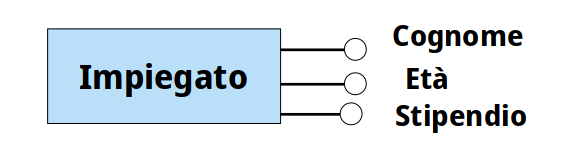
\includegraphics[width=0.75\textwidth]{2.png}
\end{center}
Se il campo è chiave, il pallino diventa pieno. (Sto odiando questa slide, è 
tutto così non simmetrico che sclero)
\section{Le Relazioni}
Una relazione (o associazione) è un legame logico tra più entità, ed il numero
di esse determina il grado (numero di entità obv), si rappresenta con un rombo
e dentro ci si scrive cosa lega le entità. Come in questo esempio:
\begin{center}
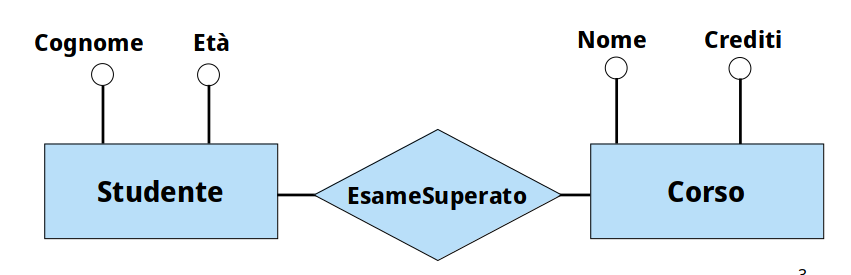
\includegraphics[width=0.75\textwidth]{3.png}
\end{center}
Siccome c'è differenza tra queste relazioni e le relazioni del modello relazionale,
per comodità le chiamerò associazioni. Quindi associazioni -> modello e-r, relazioni ->
modello relazionale.
\paragraph{Come scrivere le associazioni:} Bisogna usare dei sostantivi al 
singolare. Come da esempio: Se ho due entità studente ed esame ed in mezzo ci
metto "Supera" è sbagliato. Si deve mettere "Esame superato". (Alle superiori
ero abituato che il verbo andasse all'infinito, che ha più senso ed è più 
leggibile, ma icchè vi devo dì, noi s'attacca l'asino indoe vuole i' padrone).
\paragraph{Tra due entità posso insierire più associazioni:} Ad esempio prendendo
uno studente ed un corso, ci puoi applicare due associazioni, una può essere
"frequenZa" e l'altra boh.. "Frequenza passata". E da notare che nelle slides 
ha messo "Frequenta" e "Frequentato in passato".. Niente verbi, ovvio.
\paragraph{Anche un'associazione può avere degli attributi:} E' una proprietà
\textbf{locale} che serve ai fini dell'utente, non è una proprietà della singola
entità ma di tutte coloro che sono in legame.
\paragraph{In termini umani:} E' una funzione che associa ad ogni istanza di 
quella associazione un valore che appartiene ad un dominio dell'attributo.
\paragraph{Esempio:} Studente - \underline{superamento} - Esame, un attributo
di superamento potrebbe essere Voto. (Tra l'altro lui ha messo esameSuperato.. 
boh, diobono ok che superato è un aggettivo, ma è participio passato di superare,
queste slides sono un casino).

\end{document}